\section{Results}\label{sec:Results}

\subsection{Mortgage Classifier (Benchmark)}\label{subsec:Mortgage Classifier (Benchmark) Results}

In order to assess whether a predictive algorithm would pick up on and reproduce bias in the data, an initial classification model (as described in \textbf{chapter \ref{subsec:Model_Training_and_Prediction}} and detailed in \textbf{table \ref{tab:CH03_Model_Details}}) was trained on the HMDA dataset (see \textbf{chapter \ref{subsec:HMDA_Data}}) with the goal of predicting whether a mortgage would be granted or not for a given applicant.
The results of this model were assessed in terms of performance and fairness as described in \textbf{chapter \ref{subsec:Performance_Assessment}} and \textbf{chapter \ref{subsec:Fairness_Assessment}}, respectively.

\textbf{Performance Assessment}

When fitting the neural network to the training data, the \textit{training accuracy} of the model improved rapidly initially, leveling off after a few epochs. The \textit{validation accuracy} started at a high level and constantly improved by small increments, suggesting that both the model learning process as well as the ability to generalize to previously unseen data were successful. 
The training process was stopped by an early\_stopping callback, with the ninth epoch being the one with the least validation loss. The training results of the best epoch were:
\begin{itemize}
    \item \textit{Training Accuracy}: 0.90
    \item \textit{Validation Accuracy}: 0.90
    \item \textit{Training Loss}: 0.28
    \item \textit{Validation Loss}: 0.28
\end{itemize}
The history of the training process is depicted in \textbf{figure \ref{fig:Model_Training_History}}.

\begin{figure}
    \centering
    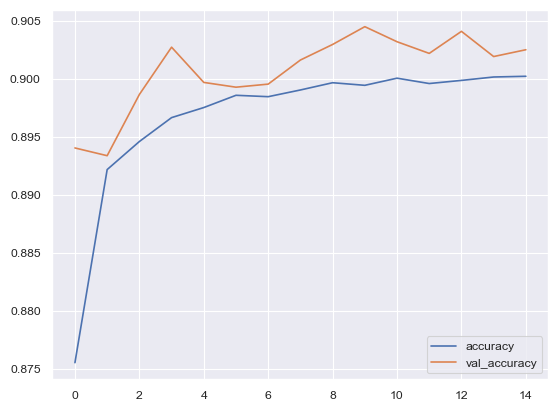
\includegraphics[width=0.85\textwidth]{images/Model_Training/Initial_Training_History.png}
    \caption{Training History of the Mortgage Classifier Model}
    \medskip
    \small
    The training history of the initial mortgage classifier model, showing the training and validation accuracy and loss over the course of the training process. The training accuracy improved constantly until the early\_stopping callback. The validation accuracy constantly improved, suggesting a successful learning process.
    \label{fig:Model_Training_History}
\end{figure}

The model was then evaluated on the test dataset, which was not seen by the model during training. The results of the performance evaluation (i.e. \textit{metrics \#1}) are shown in \textbf{table \ref{tab:Model_Evaluation}}. The model achieved an \textit{accuracy} of 0.90, a \textit{precision} of 0.88, a \textit{recall} of 0.97, and an \textit{F1-score} of 0.92. 
As stated in \textbf{chapter\ref{subsec:Performance_Assessment}}, the original model output were probabilities between 0 and 1. These could be used to calculate ROC AUC and plot the corresponding ROC curve, which can be seen in \textbf{figure \ref{fig:Model_Training_ROC}}. The \textit{ROC-AUC} score was 0.94, indicating a high level of model performance. 
Converting the probabilities into predictions with a threshold of 0.5 fulfilled the classification requirement. The \textit{confusion matrix} is depicted in \textbf{figure \ref{fig:Model_Confusion_Matrix}}. The model managed to achieve a high number of true positives and true negatives, while the number of false negatives was low. However, the number of false positives was nearly 8\% of all predictions.

\begin{table}[h]
    \centering
    \begin{tabular}{l c}
    \toprule
    \textbf{Metric} & \textbf{Value} \\
    \midrule
    \textbf{accuracy} & 0.90 \\
    \textbf{precision} & 0.88 \\
    \textbf{recall} & 0.97 \\
    \textbf{f1} & 0.92 \\
    \bottomrule
    \end{tabular}
    \caption{Metrics \#1: Initial Model}
    \small
    The mortgage classifier model was evaluated on the test dataset, achieving an accuracy of 0.90, a precision of 0.88, a recall of 0.97, and an F1-score of 0.92.
    \label{tab:Model_Evaluation}
\end{table}

\begin{figure}
    \centering
    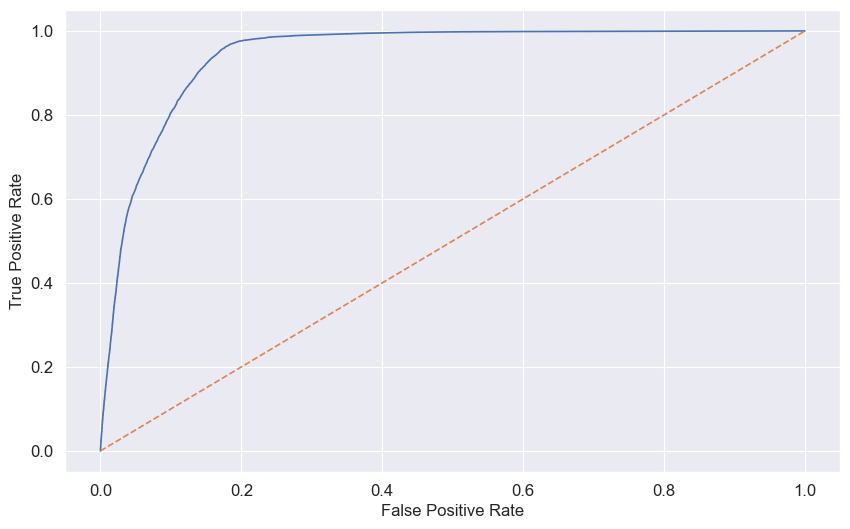
\includegraphics[width=0.85\textwidth]{images/Model_Training/Initial_ROC_curve.png}
    \caption{ROC curve of the Mortgage Classifier Model}
    \medskip
    \small
    The ROC curve is significantly above the diagonal baseline, indicating high predictive performance.
    \label{fig:Model_Training_ROC}
\end{figure}

\begin{figure}
    \centering
    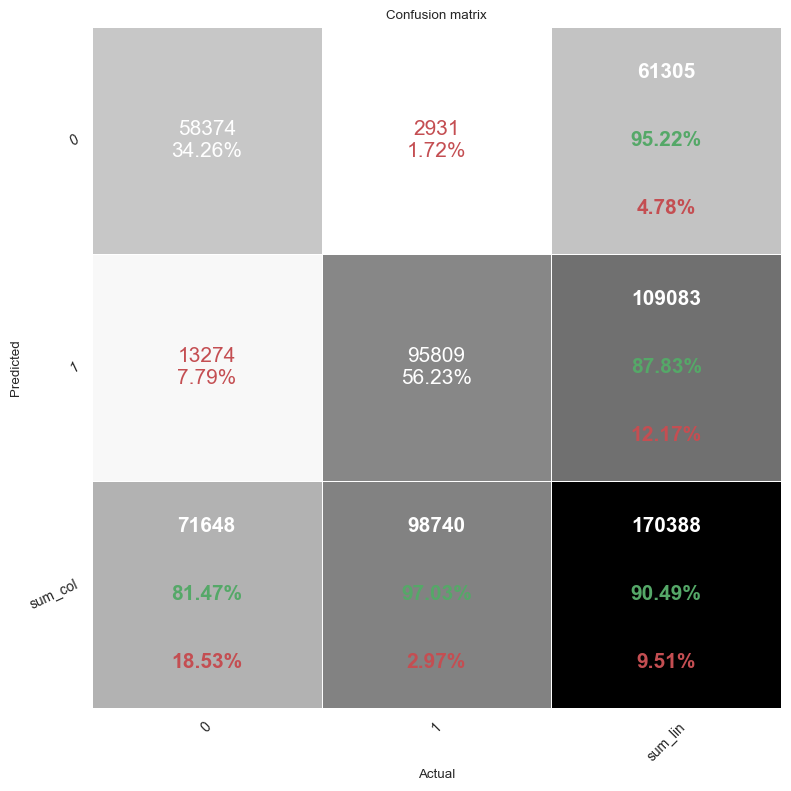
\includegraphics[width=0.85\textwidth]{images/Model_Training/Initial_Confusion_Matrix.png}
    \caption{Confusion Matrix on the Test Dataset of the Mortgage Classifier Model}
    \medskip
    \small
    The confusion matrix of the mortgage classifier model on the test dataset. The model achieved a high number of true positives and true negatives. The number of false negatives was low, however, false positives made up nearly 8\% of all predictions.
    \label{fig:Model_Confusion_Matrix}
\end{figure}

\textbf{Fairness Assessment}

Following the research question (see \textbf{chapter \ref{ch:Introduction}}), the \textit{detection of unfairness} in the predictions is an explicit goal of this thesis. To address this, the fairness assessment outlined in \textbf{chapter \ref{subsec:Fairness_Assessment}} was applied to the predictions. The results of the fairness assessment (i.e. \textit{metrics \#2}) are shown in \textbf{table \ref{tab:Fairness_Assessment_Initial}}. 
The model performed slightly better for \textit{White} applicants than for \textit{Black} applicants. The \textit{accuracy} for \textit{White} applicants was 0.91, while it was 0.88 for \textit{Black} applicants. The \textit{precision} for \textit{White} applicants was 0.89, while it was 0.82 for \textit{Black} applicants. The \textit{recall} for \textit{White} applicants was 0.97, while it was 0.96 for \textit{Black} applicants. 
The \textit{F1-score} for \textit{White} applicants was 0.93, while it was 0.88 for \textit{Black} applicants. The \textit{AUC} for \textit{White} applicants was 0.94, while it was 0.95 for \textit{Black} applicants. 
In terms of disparities (where the optimal value is \textbf{1}), the model performed comparably well in all disciplines except the \textit{fnr\_disparity}, which was 1.42. This indicates that the model was more likely to predict a false negative for \textit{Black} applicants than for \textit{White} applicants.

\begin{table}[h]
    \centering
    \begin{tabular}{lr}
    \toprule
    \textbf{Metric} & \textbf{Value} \\
    \midrule
    \textbf{Accuracy White} & 0.91 \\
    \textbf{Precision White} & 0.89 \\
    \textbf{Recall White} & 0.97 \\
    \textbf{F1 Score White} & 0.93 \\
    \textbf{AUC White} & 0.94 \\
    \midrule
    \textbf{Accuracy Black} & 0.88 \\
    \textbf{Precision Black} & 0.82 \\
    \textbf{Recall Black} & 0.96 \\
    \textbf{F1 Score Black} & 0.88 \\
    \textbf{AUC Black} & 0.95 \\
    \midrule
    \textbf{tpr\_disparity} & 0.99 \\
    \textbf{fpr\_disparity} & 0.96 \\
    \textbf{tnr\_disparity} & 1.01 \\
    \textbf{fnr\_disparity} & 1.42 \\
    \bottomrule
    \end{tabular}
    \caption{Metrics \#2: Initial Model}
    \label{tab:Fairness_Assessment_Initial}
    \small
    The benchmark model showed a slightly better performance for \textit{White} applicants than for \textit{Black} applicants. The disparities were comparably low, except for the \textit{fnr\_disparity}, which was 1.42.
\end{table}

\subsection{Explainability}\label{Explainability Results}



\textbf{SHAP}

\textbf{LIME}

\textbf{Global Surrogate Model}

\subsection{Fairness Adjustments}\label{Fairness Adjustments Results}